\chapter{Avaliação}
\label{cap:evaluation}

Neste capítulo serão apresentadas as avaliações da solução proposta, metodologias utilizadas, conjunto de dados estudados, métricas e discussões sobre o significado dos resultados em relação aos objetivos inicialmente traçados. Espera-se que com o desenvolvimento de uma métrica de similaridade semântica, explorando as relações de recursos no DBPedia\footnote{http://wiki.dbpedia.org}, seja possível tirar vantagem para sugerir itens, invés da análise mais sintática do conteúdo utilizado em métodos como \ac{TFIDF}. Também é desejado verificar o impacto do uso da sinopse do filme, um dado não estruturado, invés de itens mais comuns como gênero, diretor, atores, com o objetivo de \enquote{fugir} das recomendações que prendam mais o usuário no mesmo tipo de filmes, mas ainda assim ser capaz de ser relevante aos seus interesses.

Inicialmente serão apresentados os dados utilizados e resultados iniciais do uso da métrica de similaridade utilizada, analisando os efeitos desejados. Posteriormente o método de recomendação que utiliza a similaridade semântica apresentado na seção \ref{ssec:formula_rlws} será comparado com o método da similaridade do cosseno, utilizando-se métricas que serão definidas e apresentadas. O resultado esperado é de que utilizando um método que leve em consideração relações semânticas tenha melhores resultados daqueles que apenas possuem análises sintáticas. Por fim, serão abordadas discussões sobre resultados alcançados além de pontos de melhoria.

\section{Metodologia}
\label{sec:methodology}

Na avaliação de um sistema de recomendação é importante entender sua eficácia e seus algoritmos envolvidos, uma vez que uma análise incorreta pode levar subestimação ou superestimação da sua real precisão, como aponta \cite{Aggarwal2016:Evaluation}. Sendo assim, recomendadores podem ser avaliados tanto usando métodos denominados como \textit{online} ou \textit{offline}. Num sistema \textit{online} as opiniões e reações dos usuários são consideradas e medidas de acordo com as recomendações apresentadas, tendo sua participação de fato, como algo crucial para a compreensão dos resultados. Contudo, como a avaliação desse método requer a participação do usuário, o que nem sempre é viável, também existe o método \textit{offline}, onde um conjunto de diferentes tipos de dados históricos dos usuários são utilizados \citep{Herlocker:1999}. Para os experimentos descritos nesta seção, serão utilizados em sua maioria um conjunto de dados offline retirados do projeto MovieLens\footnote{https://movielens.org}, conforme apresentado na seção \ref{sec:av_data_set}. Utilizando-se da mesma metodologia também serão avaliados resultados de testes online, mas para um grupo bem pequeno, apenas para realizar uma comparação da diferença de resultados encontrados.

O objetivo dos experimentos que serão apresentados, é avaliar se a utilização da similaridade semântica junto ao método de recomendação proposto, é capaz de trazer resultados melhores nas métricas de avaliação em relação a similaridade do cosseno utilizando \ac{TFIDF}.  Os resultados tratam-se das análises das métricas extraídas das avaliações realizadas por usuários em relação as recomendações geradas por esses métodos.

Para realizar os testes entre os dois métodos de recomendação é necessário construir um perfil do usuário,
formado através dos filmes que avaliou. Cada usuário deve ter pelo menos 10 avaliações. Com intuito de captar os interesses do usuário, definiu-se que para montar o modelo do usuário com seus melhores termos, serão utilizados apenas os filmes com avaliação igual ou superior a 3,5, sendo 5 a avaliação máxima. No capítulo \ref{cap:proposal} foi definido que o perfil do usuário seria um conjunto $M_u$ dos melhores termos, possuindo um tamanho $z$ constante. Nos experimentos a seguir foi estipulado $z$ como 15 termos. A quantidade de termos definida possui um impacto grande na performance do sistema, uma vez que a complexidade do algoritmo da comparação entre termos é de $O(zm)$ (considerando $z$ como constante tem-se $O(m)$), sendo $m$ a quantidade de termos do filme. A Figura \ref{fig:tempo_x_termos} demonstra um gráfico da quantidade de termos do modelo do usuário em relação ao tempo de processamento, considerando que todos os dados estão no \textit{cache local}, conforme abordado no capítulo \ref{cap:proposal}, ou seja, o melhor caso.

\begin{figure}
	\centering
	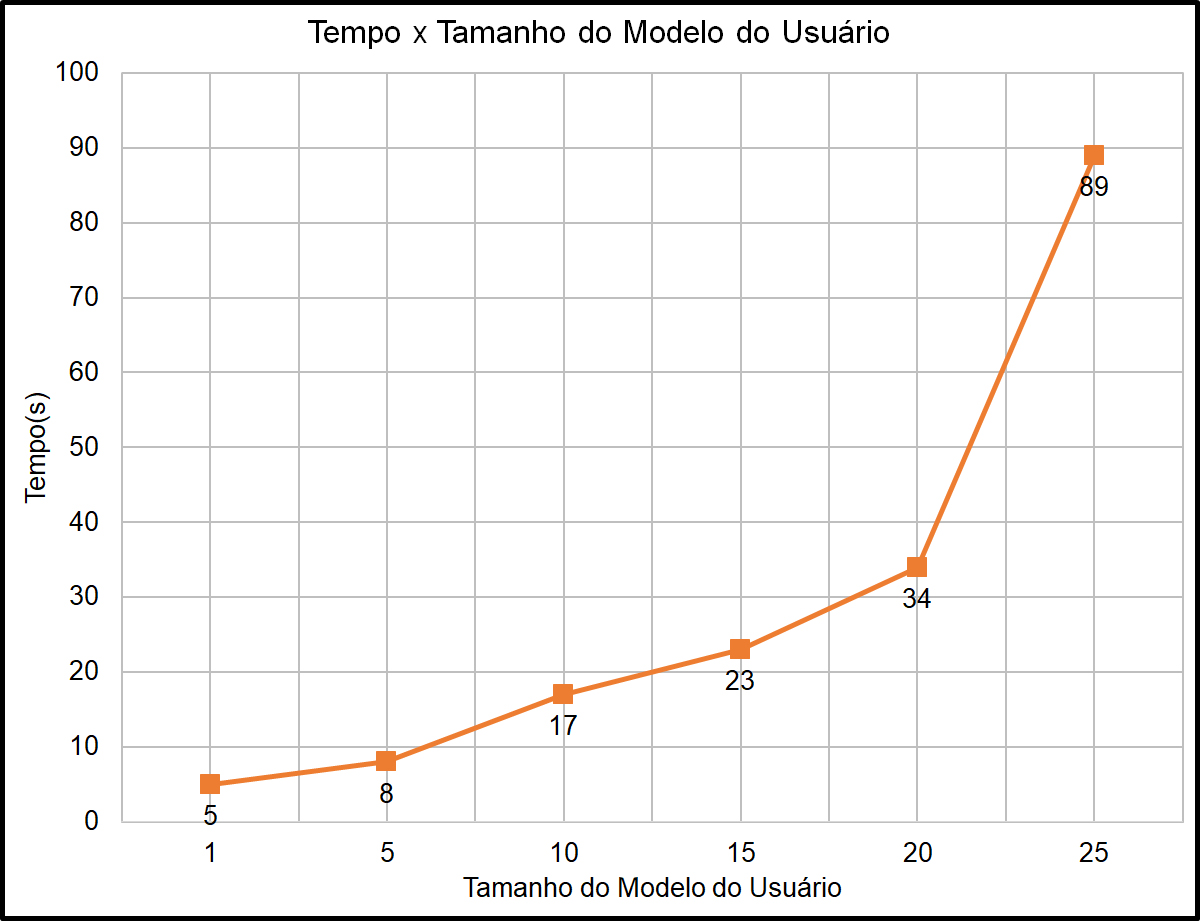
\includegraphics[scale=0.3]{imagens/tempo_x_termos.jpg}
	\caption{Gráfico da relação do tamanho do modelo do usuário (quantidade de termos usados) com o tempo de processamento para recomendação de um usuário. Todas as comparações de termos estão em \textit{cache}. Execução numa máquina com processador \textit{i7 6700K}, 16GB RAM, \textit{Windows 10}.}
	\label{fig:tempo_x_termos}
\end{figure}

Definida a metodologia para a construção do perfil do usuário, na análise dos resultados serão realizados 3 experimentos para construir as recomendações. O total de recomendações possíveis trata-se de todos os outros filmes que o usuário não avaliou, o que torna extremamente trabalhosa a sua avaliação, portando indo contrário aos propósitos de um \ac{SR}, como filtrar e classificar resultados personalizados, poupando-o tempo na busca por informações. Sendo assim, apenas uma quantidade pequena de filmes serão recomendados, sendo um total de 20 recomendações com melhores scores, por experimento, uma vez que o importante é avaliar os bons primeiros resultados, ou aqueles exibidos primeiramente, pois conforme cada vez o usuário tem que continuar procurando por resultados, pior pode ser a percepção de relevância, conforme argumentado por \cite{Manning:2008}. 

Os três experimentos consistem nas seguintes abordagens:

\begin{enumerate}
	\item{\textbf{Experimento 1}: Serão construídas recomendações utilizando o método apresentado na seção \ref{ssec:formula_rlws}, definindo os pesos como 0,8 para links diretos e 0,2 para indiretos. A seguir este experimento será referido como \textbf{RLWS DIRECT}, indicando que a prioridade nos relacionamentos diretos entre recursos.}
	\item{\textbf{Experimento 2}: Semelhante ao experimento 1, mas com pesos 0,2 para links diretos e 0,8 para indiretos. Este experimento será referido como \textbf{RLWS INDIRECT} para indicar a prioridade dos relacionamentos indiretos entre recursos.}
	\item{\textbf{Experimento 3}: Recomendações construídas utilizando o método da similaridade do cosseno, referenciada por \textbf{COSINE}.}
\end{enumerate}

O objetivo da variação dos pesos para a similaridade \ac{RLWS} é analisar o comportamento privilegiando o relacionamento direto ou indireto de recursos na DBPedia.
 
É importante ressaltar que para os testes \textit{online}, os usuários serão entrevistados, fornecendo um conjunto de 10 filmes de sua preferência, além de que não será detalhado qual método foi utilizado para as recomendações geradas por cada experimento. Para cada item recomendado o usuário terá de avaliar com uma nota de 0 a 5 estrelas, onde serão considerados os itens relevantes como aqueles que possuírem 3,5 estrelas ou mais. Já para os testes offline, como não há como saber a avaliação do usuário, será utilizada uma média das avaliações de outros usuários, onde também serão consideradas relevantes aquelas avaliações com média superior ou igual a 3,5 estrelas.

Para medir os resultados das recomendações dos experimentos serão utilizadas métricas como \textit{Precision} e \textit{Recall}, que dependem de um modelo de classificação binária \citep{Powers_2008}, sendo assim avaliações maiores ou iguais a 3,5 estrelas serão consideradas relevantes ou positivas, e inferiores como irrelevantes ou negativas. Na seção \ref{sec:av_metrics} serão melhor discutidas as métricas empregadas para avaliar os experimentos, assim como seus resultados.

Na seção seguinte será apresentado os dados trabalhados e gerados durante a execução dos experimentos.

\section{Conjunto de dados}
\label{sec:av_data_set}

Os dados usados durante os experimentos tratam-se de filmes , usuários com seus termos extraídos pelo processo do \ac{NLP}, além de avaliações. A Tabela \ref{tab:dataset} demonstra a quantidade de dados utilizados durante os testes. Note que os \enquote{URIs válidas} tratam-se termos extraídos das sinopses que possuem uma \ac{URI} associada a um recurso no DBPedia\footnote{http://wiki.dbpedia.org}. Os \enquote{usuários, teste offline} e \enquote{online} tratam-se da quantidade de usuários utilizados do total, em que foram geradas as recomendações dos experimentos.

\begin{table}[H]
\centering
\def\arraystretch{1.3}
\begin{tabular}{|l|l|}
	\hline
	\textbf{Dado}          & \textbf{Quantidades}   \\ \hline
	Filmes                 & 5.107                  \\ \hline
	Usuários               & 100.004                \\ \hline
	Usuários, teste offline & 30					\\ \hline
	Usuários, teste online & 4						\\ \hline
	Total de avaliações       & 11.997.970          \\ \hline
	Total URIs             & 22.978                 \\ \hline
	Total URIs válidas     & 18.630                 \\ \hline
	Total de comparações de URIs & 6.306.451        \\ \hline
\end{tabular}
\caption{Contagem dos dados utilizados durante os testes.}
\label{tab:dataset}
\end{table}

O total de URIs válidas é um ponto de contenção importante de ser analisado, uma vez que se o termo não se trata de um recurso na DBPedia, a comparação do \ac{RLWS} é descartada. Sendo assim, algo importante para a viabilidade da similaridade é de que a maioria dos termos extraídos das descrições dos filmes, tenha uma \ac{URI} associada ao recurso. A Tabela \ref{tab:lod_statistics} demonstra algumas estatísticas em relação aos termos extraídos dos filmes. Abaixo é descrito os conceitos construídos para a análise dos dados da tabela.

\begin{itemize}
	\item{\textbf{Cobertura DBPedia}: Trata-se do percentual dos termos encontrados que possuem uma \ac{URI} associada no DBPedia. É importante que este valor seja alto, pois caso não sejam encontrados os termos no serviço da web semântica a similaridade torna-se inválida.}
	
	\item{\textbf{Cobertura Links Diretos}: É o percentual de links que possuem pelo menos um relacionamento direto com outro termo dentro do conjunto de dados do experimento. Este valor revela o quão útil pode ser comparar dois termos quaisquer buscando por relacionamentos diretos no DBPedia, conforme abordado no capítulo \ref{cap:proposal}.}
	
	\item{\textbf{Cobertura Links Indiretos}: Similar à cobertura de links indiretos, mas agora sendo o percentual de links que possuem pelo menos um relacionamento indireto com outro termo.}
	
	\item{\textbf{Cobertura de Filmes com Links Diretos}: É o percentual de filmes contendo pelo menos um termo com ao menos um relacionamento direto a outro termo. Este valor tem o intuito de demonstrar a viabilidade da comparação utilizando a métrica \ac{RLWS} para comparar filmes utilizando-se os termos extraídos das suas descrições. A ideia é de que a maioria dos filmes possam utilizar a comparação de termos, tendo pelo menos um termo com relacionamento a outro encontrado.}
	
	\item{\textbf{Cobertura de Filmes com Links Indiretos}: O mesmo da cobertura de filmes com links diretos, mas agora sendo o percentual para os indiretos.}
\end{itemize}

\begin{table}[H]
\centering
\begin{tabular}{|l|l|}
\hline
\textbf{Dado}                           & \textbf{Valor} \\ \hline
Cobertura DBPedia                       & 81,08\%        \\ \hline
Cobertura Links Diretos                 & 21,63\%        \\ \hline
Cobertura Links Indiretos               & 64,41\%        \\ \hline
Cobertura de Filmes com Links Diretos   & 99,96\%        \\ \hline
Cobertura de Filmes com Links Indiretos & 100,00\%       \\ \hline
\end{tabular}
\caption{Estatística da cobertura dos dados dos links de recursos na DBPedia}
\label{tab:lod_statistics}
\end{table}

É importante ressaltar que os dados das coberturas apenas consideram os \enquote{links válidos}, ou seja, aqueles que possuem uma URI associada no DBPedia. Nota-se também que os dados mencionados na tabela em relação a cobertura de links diretos e indiretos trata-se das comparações realizadas nos experimentos, sendo assim, não se completam, pois ainda existem links com relacionamentos que não foram comparados.

Algo relevante para destacar quanto à relação entre recursos é de que a quantidade de relacionamentos entre recursos cujo a quantidade links diretos é maior que 0, é de aproximadamente 0,12\% em relação ao total de relações entre recursos, conforme constatado na Tabela \ref{tab:lod_cache_stats}. Já era esperado que a maioria dos recursos não tivesse propriedades diretamente conectadas entre si, devido a variedade de comparações indiscriminada entre termos do usuário e termos dos filmes. Isso resulta numa tabela de dados altamente esparsa em relação ao cálculo a participação direta na equação \ac{RLWS}, o que por consequência leva a uma tabela de dados grande contendo diversas comparações zeradas. Quanto a proporção de relacionamentos indiretos maiores que 0 em relação ao total é de aproximadamente 8,05\%. Embora esses valores sejam baixos, o foco é de que para cada termo existam pelo menos um relacionamento a outro termo, seja direta ou indiretamente, e de que esse relacionamento esteja distribuído pela maioria dos filmes, algo que é evidenciado pelos dados da Tabela \ref{tab:lod_statistics}. Na tabela abaixo ainda são apresentados os de recursos relacionados que possuem a propriedade \textit{dbo:wikiPageRedirects}, ou seja, aqueles que o DBPedia resolve sua \ac{URI} como sendo a mesma, portanto para a similaridade considerados iguais.

\begin{table}[H]
\centering
\def\arraystretch{1.3}
\begin{tabular}{|l|l|}
\hline
\textbf{Dado}                                   & \textbf{Quantidades} \\ \hline
Relação entre recursos                          & 6.306.451            \\ \hline
Relação entre recursos, direto $> 0$ 			& 7.977                \\ \hline
Relação entre recursos, indireto $> 0$ 			& 510.533              \\ \hline
Relação entre recursos, redirecionados entre si & 194                  \\ \hline
Relação entre recursos, direto e indireto $= 0$ & 5.794.914            \\ \hline
\end{tabular}
\caption{Contagem da relação entre recursos utilizados durante os experimentos.}
\label{tab:lod_cache_stats}
\end{table}

\section{Métricas de avaliação}
\label{sec:av_metrics}

Existem diversas métricas que são usadas tanto em avaliações \textit{online} e \textit{offline}, mas as mais comuns são as de \textit{accuracy}, embora existam outras como \textit{user coverage}, \textit{novelty}, \textit{trust} \citep{Jannach:2010}. Para este trabalho foram utilizadas tanto avaliações \textit{online} e \textit{offline}, com métodos de precisão para avaliar as classificações da recomendações, como \textit{Precision} e \textit{Recall}. Abaixo serão abordados os conceitos das métricas de avaliação utilizadas nos experimentos.

\subsection{Precision}

Avaliando recomendações com métodos \textit{offline} apenas utilizando dados históricos da preferência do usuário, somente pode informar aqueles itens que foram de conhecimento do usuário, portando todos os outros itens terão de avaliados de outras formas, que não seja diretamente pela sua opinião, o que pode levar à falso positivos e/ou negativos. Por outro lado, avaliando com usuários reais, esses podem julgar todos os itens recomendados, podendo de fato definir se a predição foi correta ou não. Com a avaliação do usuário é possível construir uma tabela de classificação conforme a Figura \ref{fig:truth_table} \citep{Jannach:2010}, onde há o cruzamento entre o que o recomendador apresentou e o que usuário avaliou. Se um item foi apresentado na recomendação e o usuário tenha gostado, avaliado como relevante, tem-se um caso de predição correta, ou \textit{true positive}. Outro resultado positivo, trata-se de quando o usuário não tenha gostado e o recomendador omitiu o resultado, ou seja uma omissão correta ou \textit{true negative}. Assim os resultados positivos estão na diagonal da esquerda para direita da tabela, e os resultados não desejados e negativos estão na outra diagonal. 

\begin{figure}
	\centering
	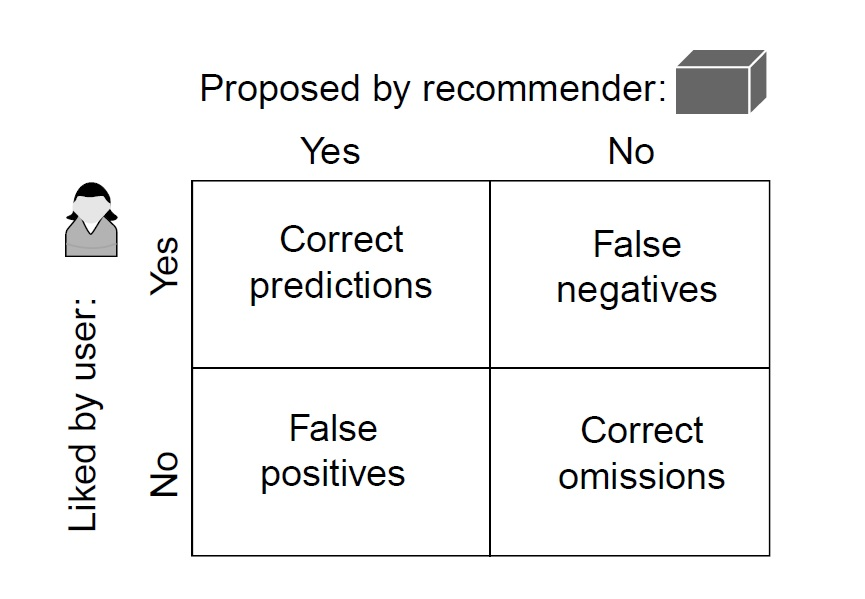
\includegraphics[scale=0.4]{imagens/truth_table.jpg}
	\caption{Tabela de tipos de erros baseada na ilustração de \cite{Jannach:2010}.}
	\label{fig:truth_table}
\end{figure}

Considerando e classificando os resultados dessa forma binária, em positivos e negativos, defini-se \textit{precision}, precisão ou confiança, como sendo a fração de resultados previstos e avaliados pelo usuário como positivos, ou seja, os \textit{true positive}, em relação a quantidade de todos os itens recomendados \citep{Powers_2008}. A Equação \ref{eq:precision} demonstra o cálculo da precisão $P$, onde $tp$ trata-se da quantidade de itens \textit{true positive} e $fp$ como \textit{false positive}.

\begin{equation}
	P = \frac{tp}{tp + fp}
\label{eq:precision}
\end{equation}

Como a quantidade de resultados pode ser muito grande para calcular a precisão, e até para que o próprio usuário o faça, por extensão também defini-se como $P@k$, como sendo a precisão até $k$ primeiros resultados retornados pelo recomendador \citep{Aggarwal2016:Evaluation}. A Equação \ref{eq:precision_at_k} demonstra a variação do cálculo de $P$ onde $r$ trata-se da quantidade de itens relevantes até o \textit{rank} $k$. \ref{eq:precision_at_k}.

\begin{equation}
	p@k = \frac{r}{k}
\label{eq:precision_at_k}
\end{equation}

\subsection{Mean Average Precision (MAP)}

Outra métrica de precisão trata-se da \ac{MAP}, que busca estipular um único valor de precisão em relação ao conjunto de avaliações de múltiplos usuários \citep{Manning:2008}. A equação \ref{eq:map} demonstra o cálculo, onde $AveP(u)$ trata-se da média das precisões $p@k$ do usuário $u \in U$, onde $|R|$ é quantidade de itens relevantes até $k$-ésimo \textit{rank}. Posteriormente obtém-se o $MAP$ como sendo a média $AveP$ para todos os usuários avaliados. A Figura \ref{fig:map_ex} exemplifica o cálculo da métrica, onde os quadrados \enquote{verdes} representam os itens \textit{true positive} e os itens vermelhos os \textit{false positive}.

\begin{equation}
	AveP(u) = \frac{\sum_{k=1}^{n} p@k}{|R|}, \; u \in U
\label{eq:avep}
\end{equation}

\begin{equation}
	MAP = \frac{\sum_{u=1}^{|U|}AveP(u)}{|U|}
\label{eq:map}
\end{equation}

\begin{figure}
	\centering
	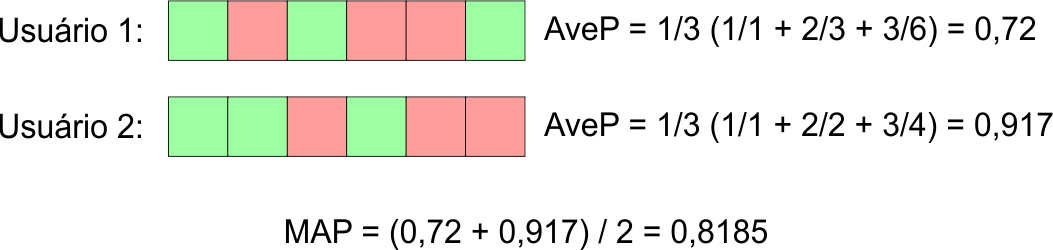
\includegraphics[scale=0.4]{imagens/map_ex.jpg}
	\caption{Exemplo do cálculo do MAP.}
	\label{fig:map_ex}
\end{figure}

\subsection{Mean Reciprocal Rank (MRR)}

A métrica \ac{MRR} trata-se da média da classificação recíproca (\textit{reciprocal rank}) de cada usuário \citep{Burges:2006}, sendo esta o multiplicativo inverso a posição do primeiro item correto no \textit{rank} de recomendações, ou top-N itens. O objetivo é obter um valor geral que informe o quão longe o primeiro resultado positivo está do primeiro item. A Equação \ref{eq:mrr} demonstra o cálculo onde $\frac{1}{k}$ trata-se do \textit{reciprocal rank} até o $k$-ésimo item. A Figura \ref{fig:mrr_ex} exemplifica o cálculo da métrica, onde os quadrados \enquote{verdes} representam os itens \textit{true positive} e os itens vermelhos os \textit{false positive}.

\begin{equation}
	MRR = \frac{1}{|U|} \sum_{u=1}^{|U|} \frac{1}{k}, \; u \in U
\label{eq:mrr}
\end{equation}

\begin{figure}
	\centering
	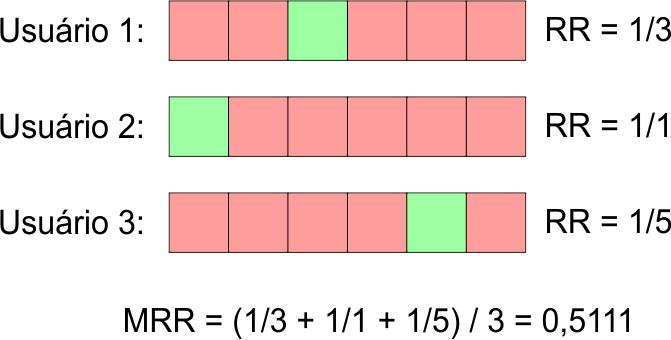
\includegraphics[scale=0.4]{imagens/mrr_ex.jpg}
	\caption{Exemplo do cálculo do MRR.}
	\label{fig:mrr_ex}
\end{figure}

\section{Resultados}
\label{sec:results}

Antes de apresentar os resultados das recomendações com as avaliações dos usuários, é importante avaliar algumas premissas e comportamentos da própria equação de similaridade, a \ac{RLWS}. Inicialmente o esperado é de que recursos que sejam intuitivamente próximos, ou provavelmente tenham diversas relações entre si,  como \textit{Earth} e \textit{Moon}, possuam maior similaridade do que \textit{Earth} e \textit{Table}. E de fato, mesmo nos dois extremos de pesos, seja priorizando as links diretos ou indiretos, existe uma diferença considerável quando termos estão intuitivamente mais próximos do que aqueles que provavelmente não terão relacionamentos em comum, conforme mostra Figura \ref{tab:rlws_results}. É importante ressaltar que \enquote{RLWS DIRECT} refere-se à configuração de pesos $w_d = 0,8, w_i = 0,2$, enquanto que \enquote{RLWS INDIRECT} é o inverso, assim priorizando os relacionamentos indiretos entre dos termos.

\begin{table}[H]
\centering
\begin{tabular}{|l|l|l|l|}
\hline
\textbf{Termo 1} & \textbf{Termo 2}    & \textbf{RLWS DIRECT} & \textbf{RLWS INDIRECT} \\ \hline
France           & Paris               & 0,434                   & 0,858                   \\ \hline
France           & Juice               & 0,111                   & 0,443                   \\ \hline
France           & Art                 & 0,190                   & 0,760                   \\ \hline
Brazil           & Brasilia            & 0,193                   & 0,770                   \\ \hline
Brazil           & Box                 & 0,050                   & 0,200                   \\ \hline
Brazil           & Paper               & 0,163                   & 0,652                   \\ \hline
Brazil           & Beach               & 0,282                   & 0,726                   \\ \hline
Car              & Automobile          & 1,0                     & 1,0                     \\ \hline
United\_States   & Washington,\_D,C,   & 0,372                   & 0,842                   \\ \hline
China            & Hong\_Kong          & 0,377                   & 0,842                   \\ \hline
Ariana\_Grande   & Selena\_Gomez       & 0,320                   & 0,800                   \\ \hline
Selena\_Gomez    & Elon\_Musk          & 0,022                   & 0,087                   \\ \hline
Coconut          & Plant               & 0,393                   & 0,683                   \\ \hline
Tom\_Cruise      & Lady\_Gaga          & 0,162                   & 0,646                   \\ \hline
Star             & Galaxy              & 0,339                   & 0,809                   \\ \hline
Earth            & Moon                & 0,485                   & 0,866                   \\ \hline
Earth            & Table               & 0,033                   & 0,132                   \\ \hline
Book             & Movie               & 0,125                   & 0,500                   \\ \hline
Book             & Metal               & 0,096                   & 0,386                   \\ \hline
Johnny\_Cash     & June\_Carter\_Cash  & 0,579                   & 0,868                   \\ \hline
Johnny\_Cash     & Al\_Green           & 0,176                   & 0,705                   \\ \hline
Johnny\_Cash     & Elvis\_Presley      & 0,316                   & 0,816                   \\ \hline
Johnny\_Cash     & Kris\_Kristofferson & 0,317                   & 0,804                   \\ \hline
Johnny\_Cash     & Carlene\_Carter     & 0,457                   & 0,743                   \\ \hline
\end{tabular}
\caption{Tabela de amostra de comparações entre termos usando \ac{RLWS}.}
\label{tab:rlws_results}
\end{table}

É importante ressaltar que mesmo para termos que estejam aparentemente mais distantes, como \textit{Selena\_Gomez} e \textit{Ariana\_Grande}, por se tratarem de "coisas" que não são imediatamente próximas, ainda possuem uma alta similaridade, devido as conexões que ambas as pessoas possuem quanto ao domínio da música e aparições em temas de filmes, programas etc. Já quando compara-se \textit{Selena\_Gomez} com \textit{Elon\_Musk}, mesmo também sendo uma comparação entre pessoas, já possuem uma similaridade bem menor, o que também é intuitivamente esperado. Também se observa na comparação \textit{Johnny\_Cash} e \textit{June\_Carter\_Cash}, uma alta similaridade, pois os dois foram casados e cantores. Outra observação importante é quanto aos termos \textit{Car} e \textit{Automobile} que possuem similaridade 1. Isso é devido que os dois possuem a propriedade \textit{dbo:wikiPageRedirect} conectando seus recursos, o que por regra na equação terá valor 1. Esses redirecionamentos também ocorrem nos termos \textit{Future} e \textit{Futuristic}, \textit{Power} e \textit{Powerful} entre outros. Para uma série de termos esses redirecionamentos contribuem para o desempenho da equação, devido a sua real proximidade, apesar de serem termos diferentes.

Nota-se que intuitivamente os resultados das comparações fazem sentido tanto usando pesos que privilegiam links diretos ou indiretos, o que é vital para coerência no momento da comparação termo a termo. Outro fato importante é a consideração de itens que possuem redirecionamentos, ainda que sejam raros, mas para palavras como "Carro" e "Automóvel" é sensato dizer que são similares.

Avaliadas as premissas e os resultados para a similaridade semântica proposta, em sequência serão calculados as métricas mencionadas na seção \ref{sec:av_metrics}, medindo assim o impacto do modelo de recomendação assim como a própria similaridade \ac{RLWS}. Os testes dos experimentos mencionados na seção \ref{sec:methodology} serão divididos em dois resultados, os testes com dados de \enquote{usuários offline} e \enquote{usuários offline}.

\subsection{MAP}

Para medir a assertividade do \ac{SR} foi utilizada a métrica \ac{MAP} perante dois conjuntos de usuários, os dos testes \textit{offline} (sendo no total de 30) e os \textit{online} (com total de 4). As Figuras \ref{fig:map_line} e \ref{fig:map_box_plot} apresentam os resultados obtidos nos três experimentos, tanto para os testes online quanto para os offline. 

O mais notável dos valores obtidos é o fato de que os testes do experimento 2, com \textit{RLWS INDIRECT}, teve um desempenho consideravelmente melhor que os outros nos dois testes, em especial a seu par que privilegia os links diretos, sendo 51\% superior (0,532 contra 0,351) ao \textit{COSINE} para um conjunto de cinco itens ($k=5$) nos testes \textit{offline}. Quanto aos resultados utilizando a métrica \textit{RLWS DIRECT}, há uma divergência entre os testes das Figuras \ref{fig:map_line_a} e \ref{fig:map_line_b}, sendo que o primeiro teste obteve um desempenho próximo à métrica \textit{COSINE}, na verdade até perdendo, enquanto que nos testes \textit{offline} ganha em 27\% (0,447 contra 0,351) para os itens até o \textit{rank} 5. Nos testes offline ambas as variantes \ac{RLWS} obtiveram um desempenho consideravelmente superior à similaridade do cosseno, já para os testes \textit{online} o maior destaque vai para o experimento 2, com \textit{RLWS INDIRECT}.

Mesmo com um desempenho inferior, o experimento \textit{RLWS DIRECT} obteve um resultado próximo da similaridade do cosseno nos testes online, o que indica que com um peso um pouco menor para os relacionamentos diretos como $w_d = 0,65, w_i = 0,35$, pode-se obter melhores resultados. A influencia dos relacionamentos diretos é esperada que tenha um impacto menor numa visão geral, devido a improbabilidade de um termo possuir tal conexão com outro, conforme é evidenciado pelas estatísticas apresentadas nas Tabelas \ref{tab:lod_statistics} e \ref{tab:lod_cache_stats}. Outra observação importante é que para os 5 primeiros itens as duas métricas \ac{RLWS} possuem uma maior precisão, o que pode ser notado tanto para os limites superiores e \textit{outliers} nas Figuras \ref{fig:map_box_plot_a} e \ref{fig:map_box_plot_b}.

\begin{figure}
    \begin{subfigure}{.5\textwidth}
        \centering
        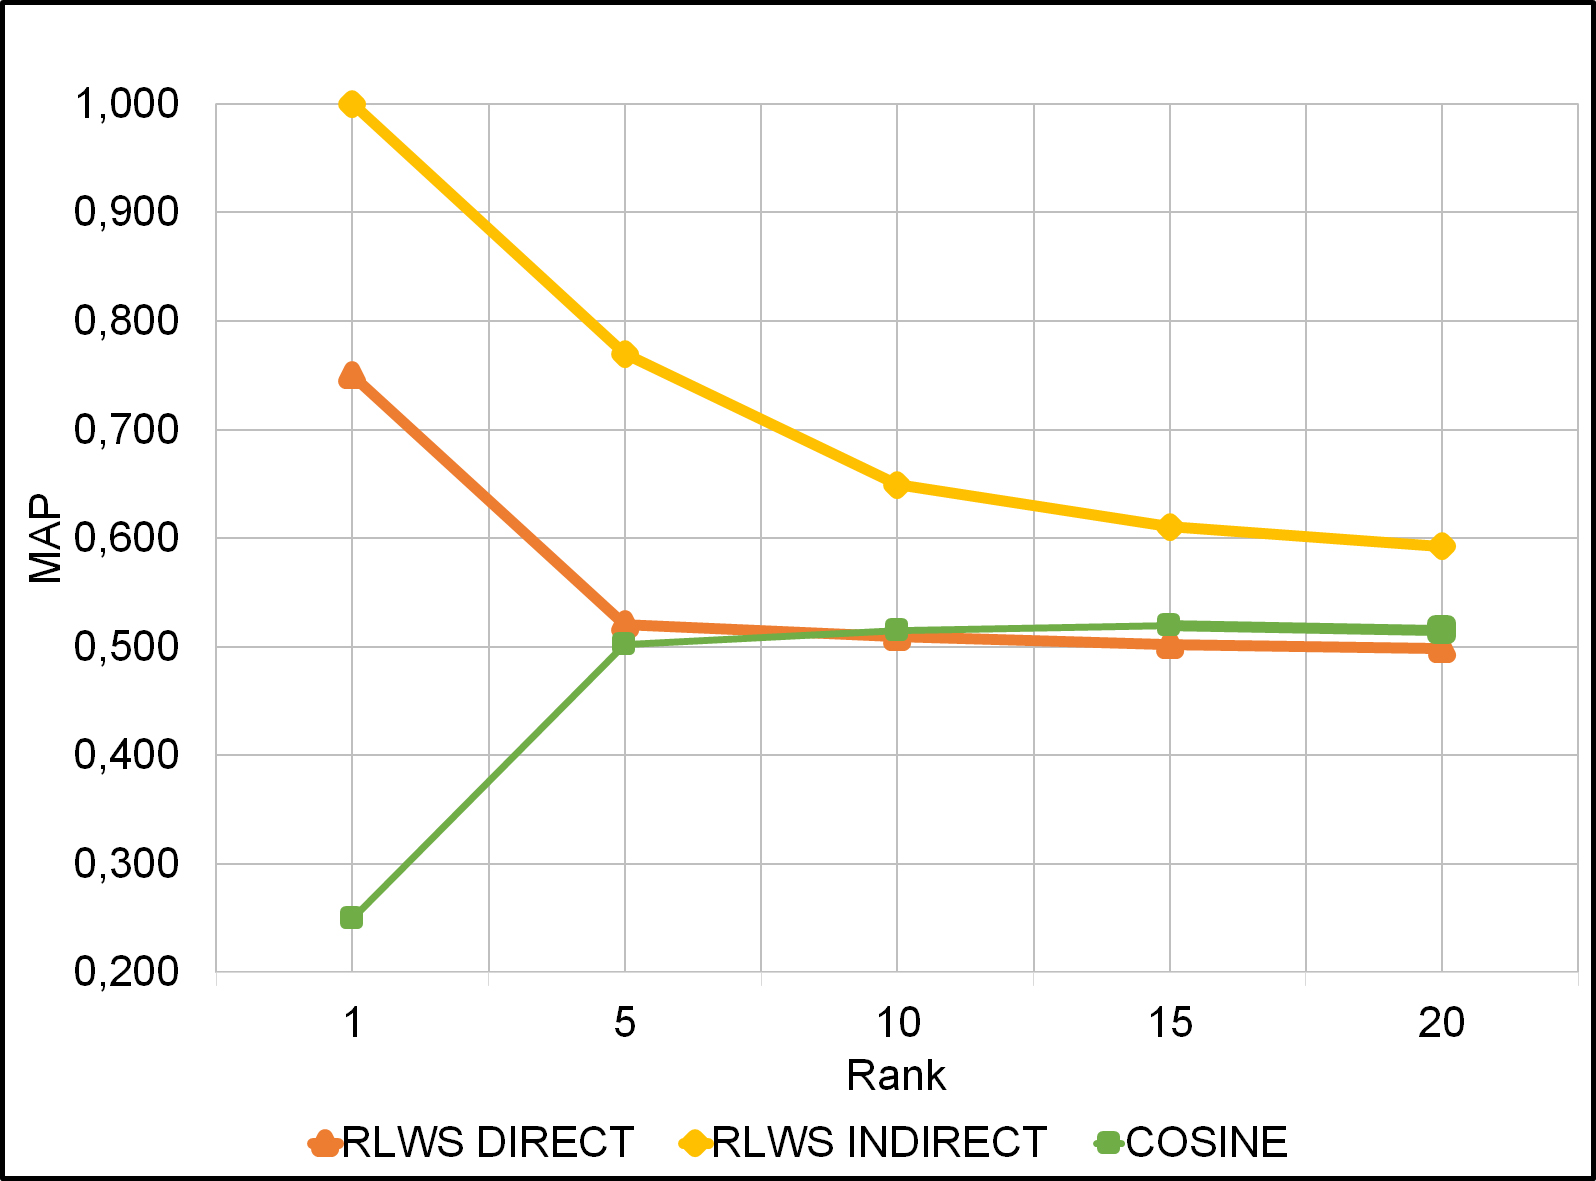
\includegraphics[width=.8\linewidth]{imagens/map_results_online.jpg}
        \caption{testes online}
        \label{fig:map_line_a}
    \end{subfigure}%
    \begin{subfigure}{.5\textwidth}
        \centering
        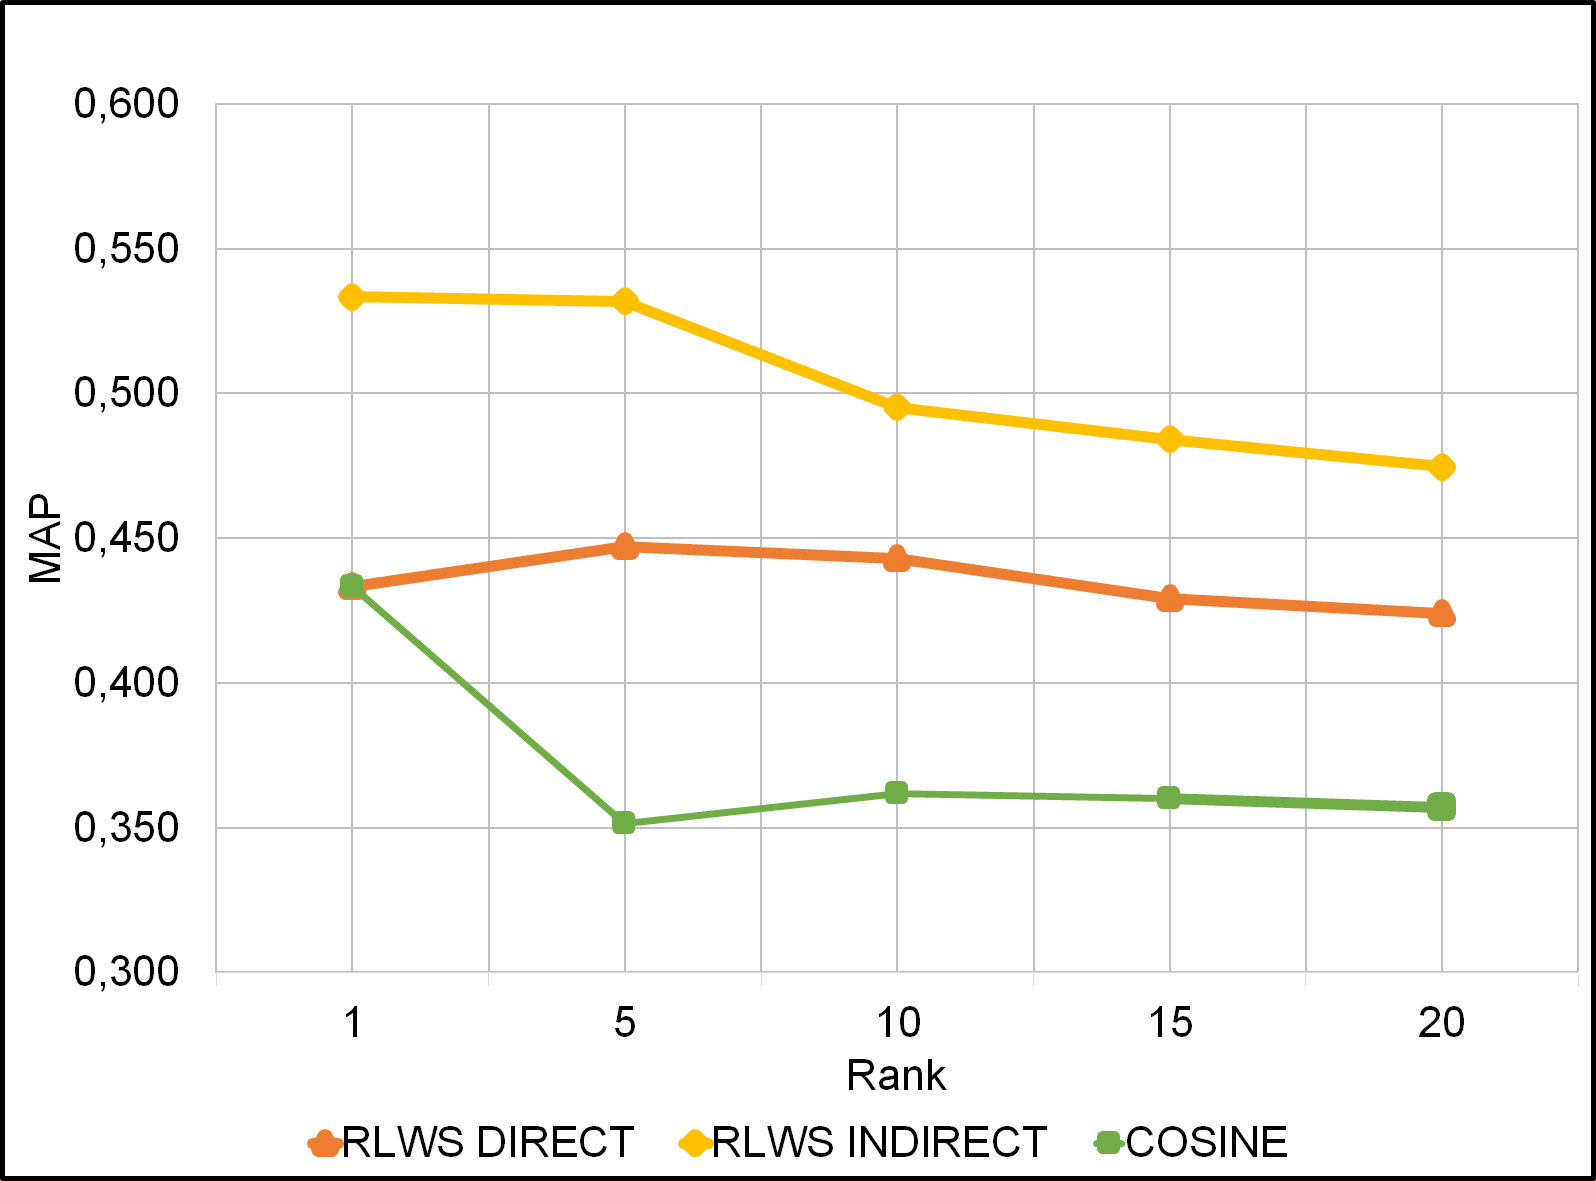
\includegraphics[width=.8\linewidth]{imagens/map_results_offline.jpg}
        \caption{testes offline}
        \label{fig:map_line_b}
    \end{subfigure}
    \caption{MAP - Gráfico com linhas dos três experimentos nos testes online e offline}
    \label{fig:map_line}
\end{figure}

\begin{figure}
    \begin{subfigure}{.5\textwidth}
        \centering
        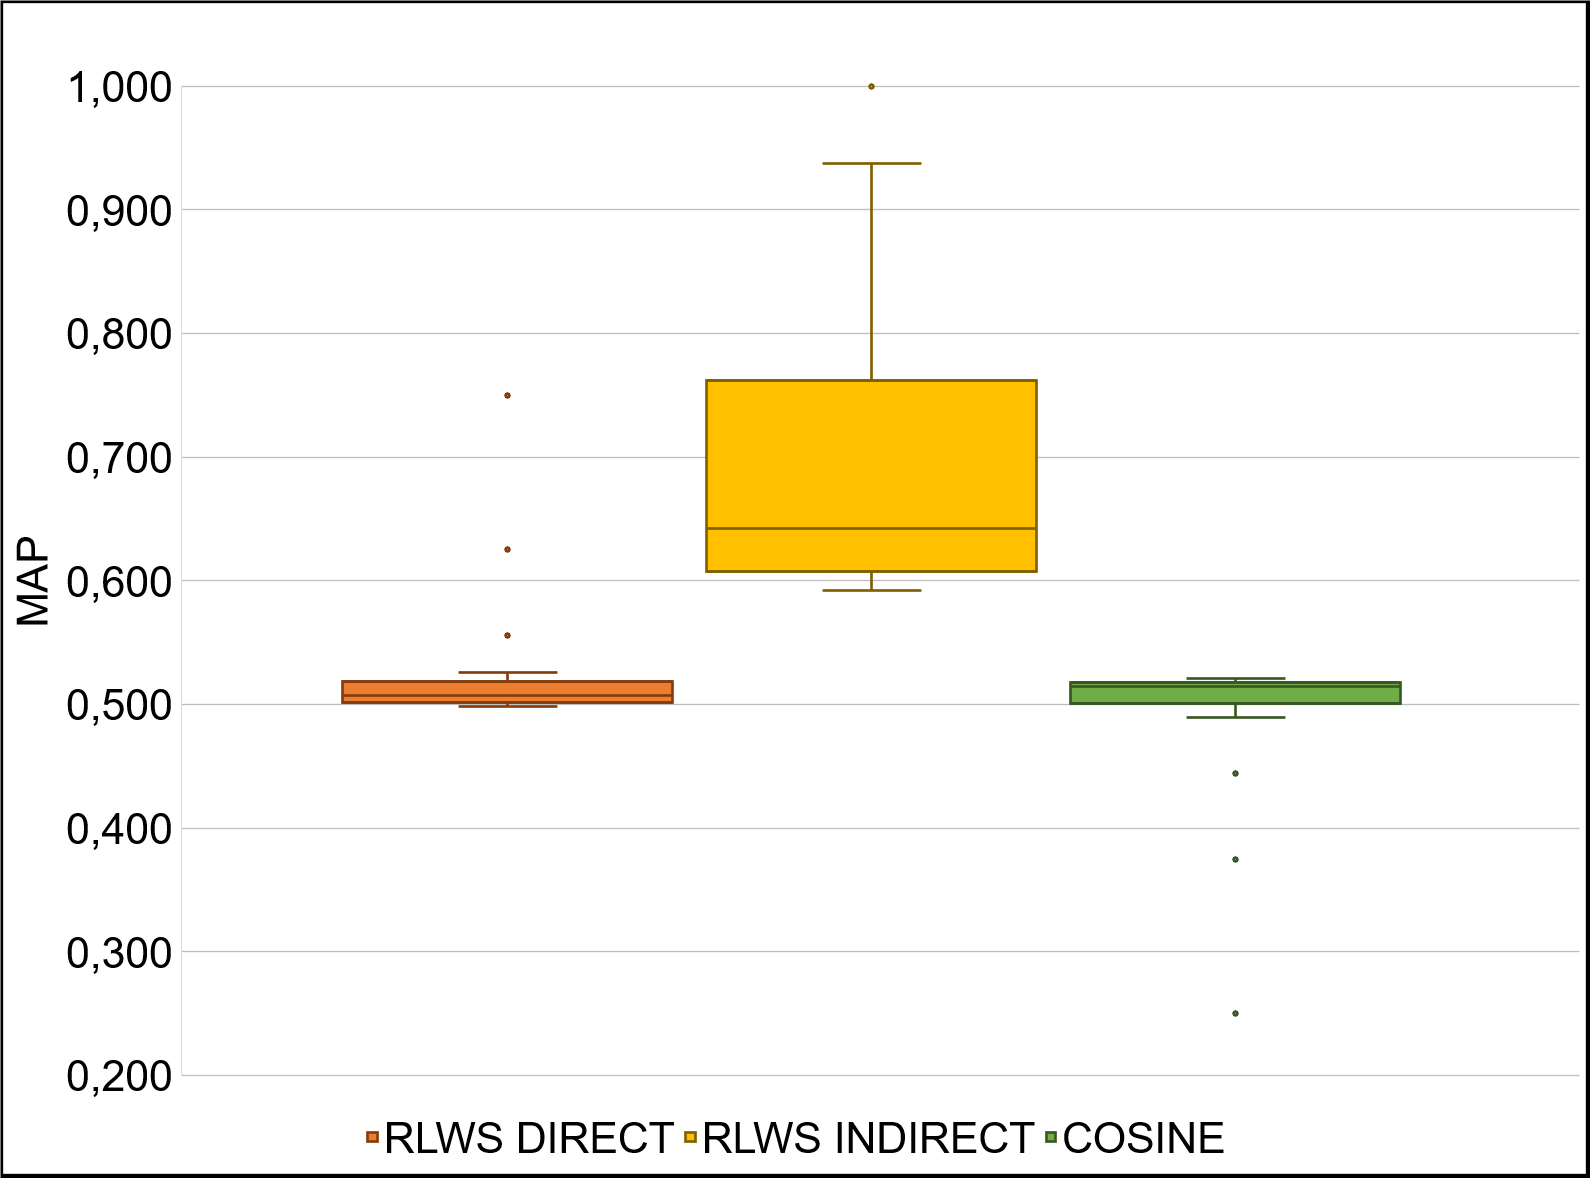
\includegraphics[width=.8\linewidth]{imagens/map_box_plot_online.jpg}
        \caption{testes online}
        \label{fig:map_box_plot_a}
    \end{subfigure}%
    \begin{subfigure}{.5\textwidth}
        \centering
        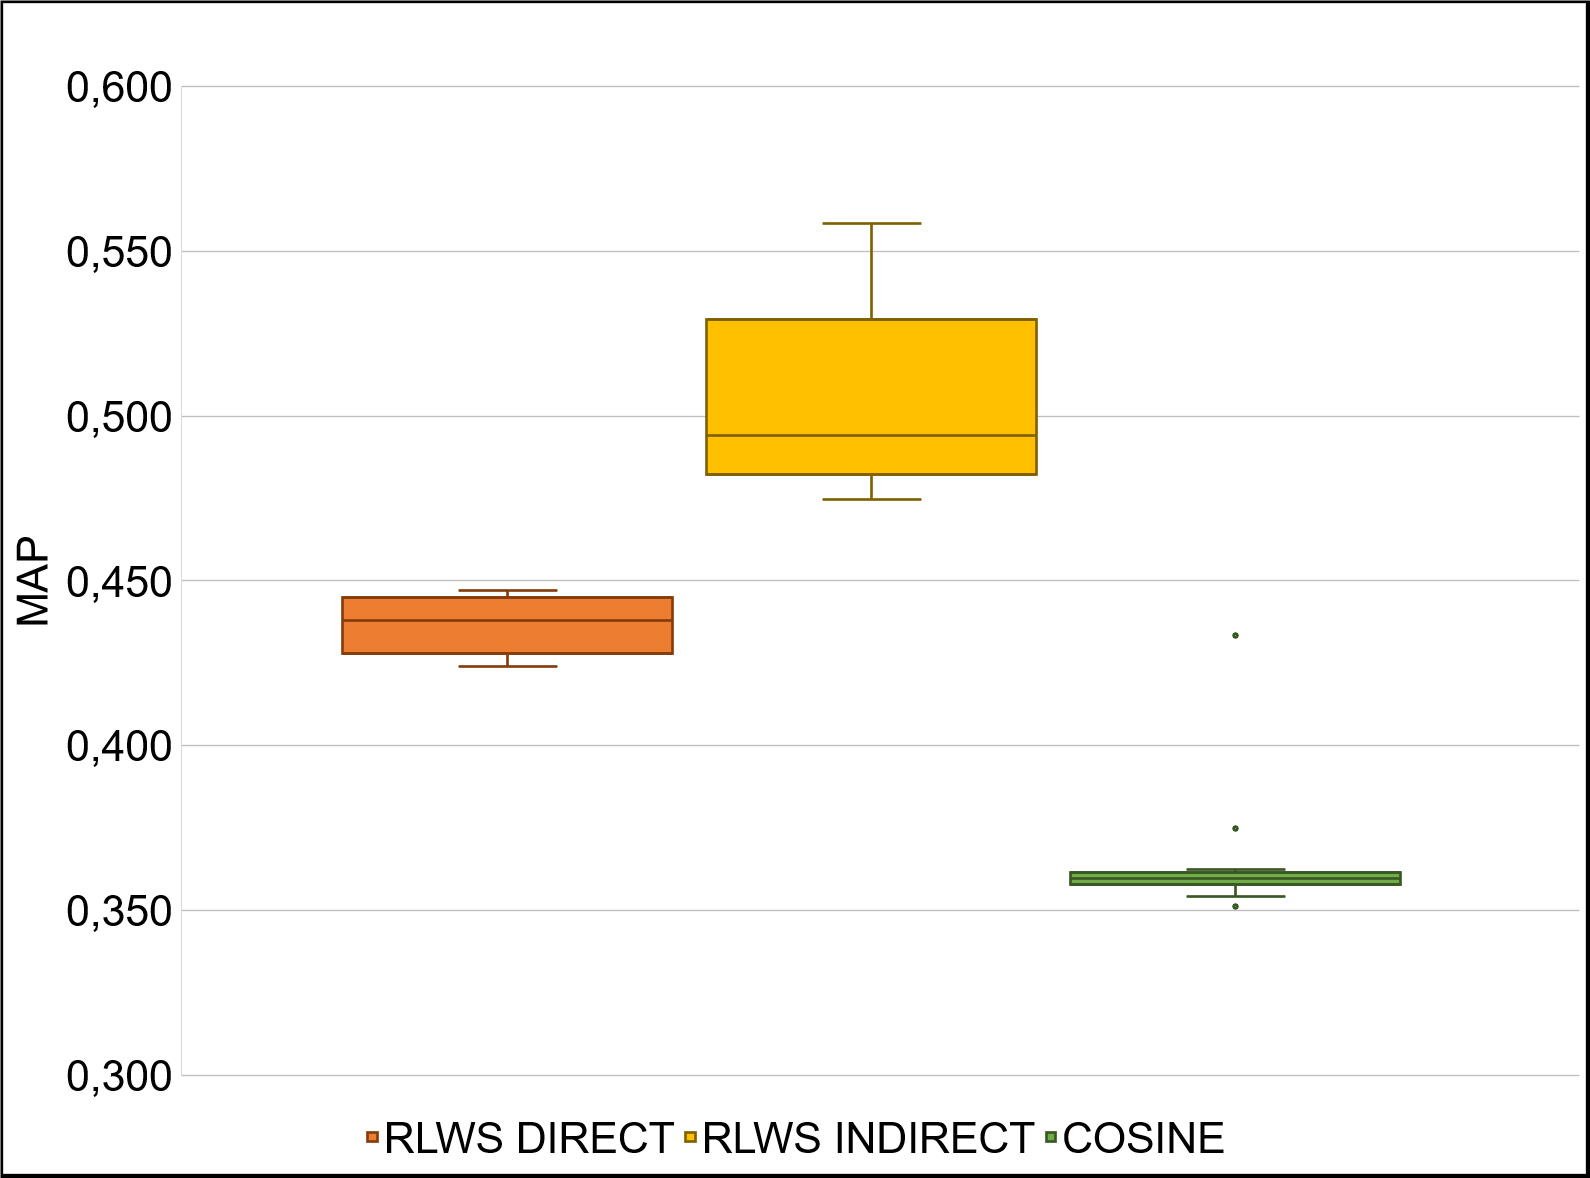
\includegraphics[width=.8\linewidth]{imagens/map_box_plot_offline.jpg}
        \caption{testes offline}
        \label{fig:map_box_plot_b}
    \end{subfigure}
    \caption{MAP - Gráfico de caixa dos três experimentos nos testes online e offline}
    \label{fig:map_box_plot}
\end{figure}

\subsection{MRR}

Para avaliar a objetividade do \ac{SR} foi utilizada a métrica \ac{MRR} perante dois conjuntos de usuários, os dos testes \textit{offline} (sendo no total de 30) e os \textit{online} (com total de 4). As Figuras \ref{fig:mrr_line} e \ref{fig:mrr_box_plot} apresentam os resultados obtidos nos três experimentos para ambos os testes. 

Assim como na métrica \ac{MAP}, também é possível observar um desempenho consideravelmente superior para o experimento 2 com a similaridade \textit{RLWS INDIRECT}, sendo 26\% (0,724 contra 0,574) superior a similaridade do cosseno nos testes \textit{offline}, para os 5 primeiros itens. Quanto ao outro par \textit{RLWS DIRECT}, obteve um resultado 11\% (0,637 contra 0,574) superior nos testes \textit{offline}. Nota-se que na Figura \ref{fig:mrr_line_a} tem-se uma linha reta com a maior nota possível, indicando que para todos os usuários nos testes online, um resultado positivo foi encontrado logo no primeiro item recomendado. Já para os testes offline é possível observar que para ambos os experimentos da métrica \ac{RLWS} foram encontrados resultados positivos já no primeiro item para mais da metade dos usuários, com o experimento \textit{COSINE} ficando um pouco abaixo. 

Os gráficos de caixa aparentes nas Figuras \ref{fig:mrr_box_plot_a} e \ref{fig:mrr_box_plot_b}, possuem em sua maioria apenas linhas retas juntamente com os \textit{outliers} devido ao fato de que a partir da 5º posição não há muito mais usuários que ainda não obtiveram uma recomendação positiva.

\begin{figure}
    \begin{subfigure}{.5\textwidth}
        \centering
        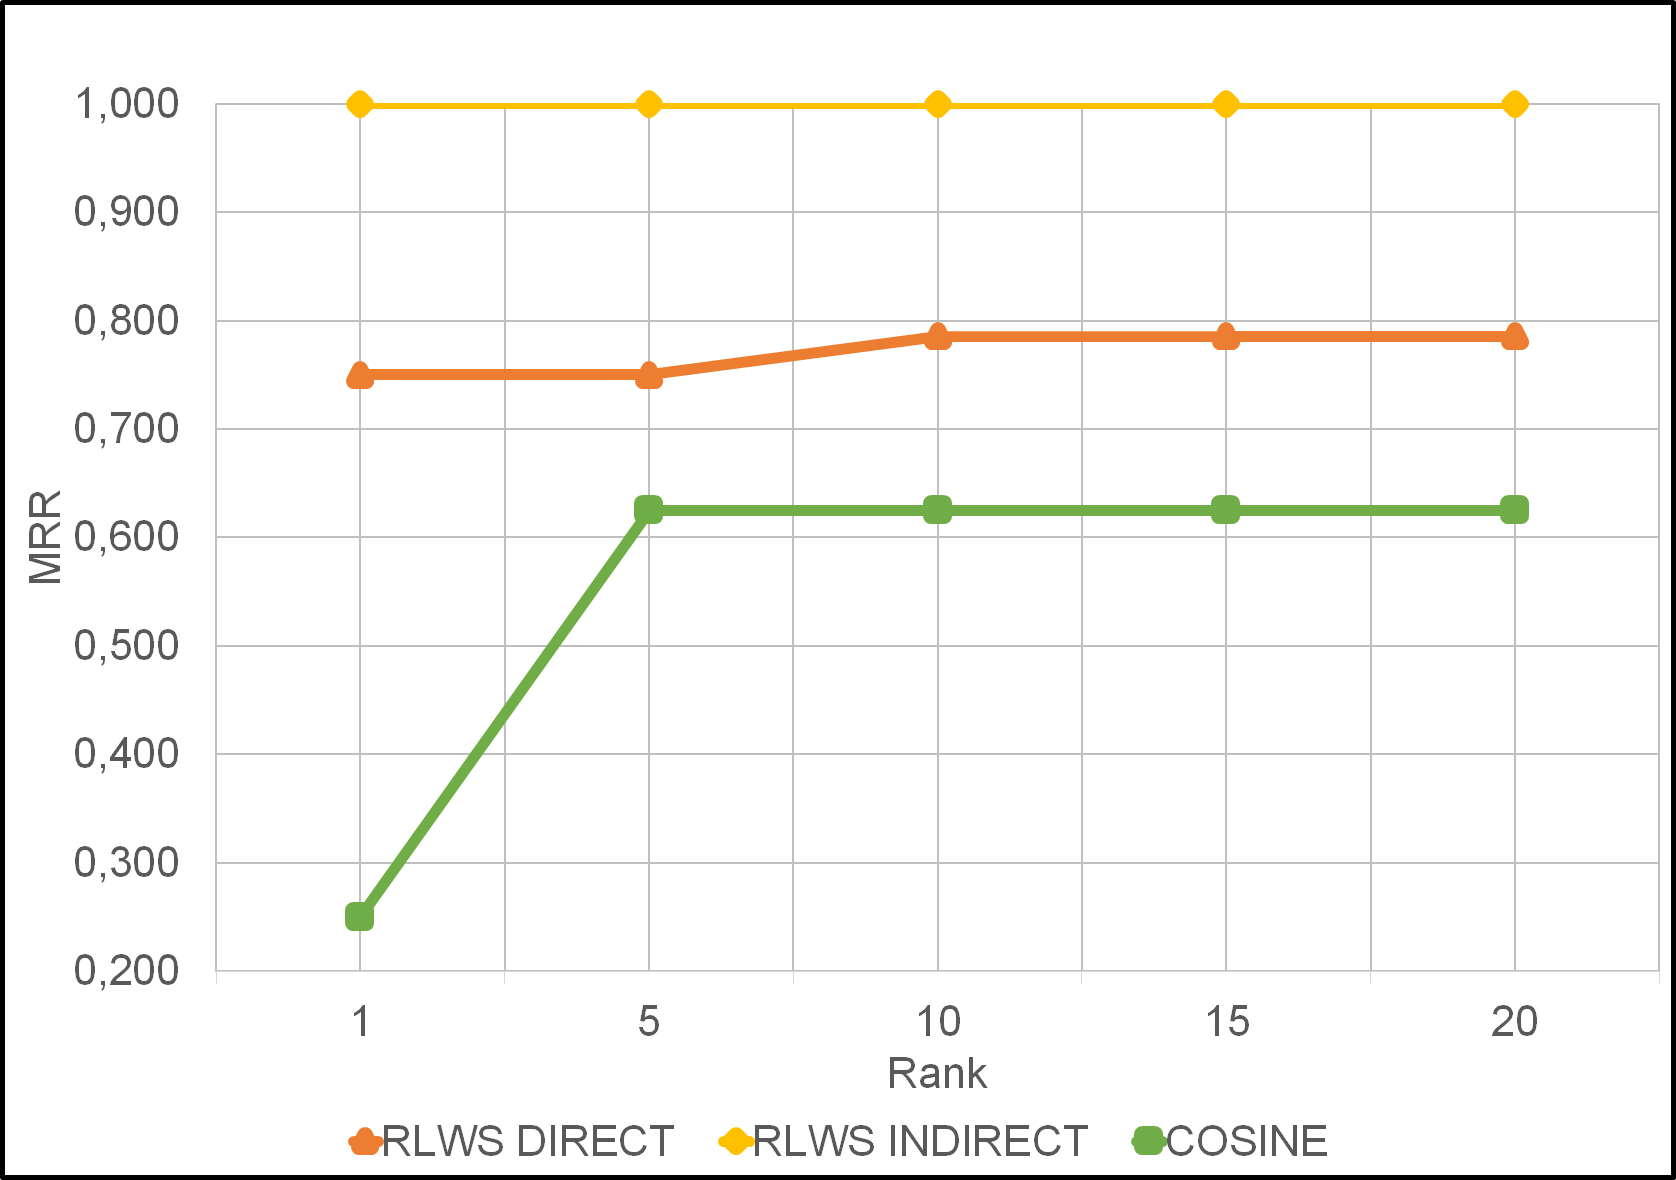
\includegraphics[width=.8\linewidth]{imagens/mrr_results_online.jpg}
        \caption{testes online}
        \label{fig:mrr_line_a}
    \end{subfigure}%
    \begin{subfigure}{.5\textwidth}
        \centering
        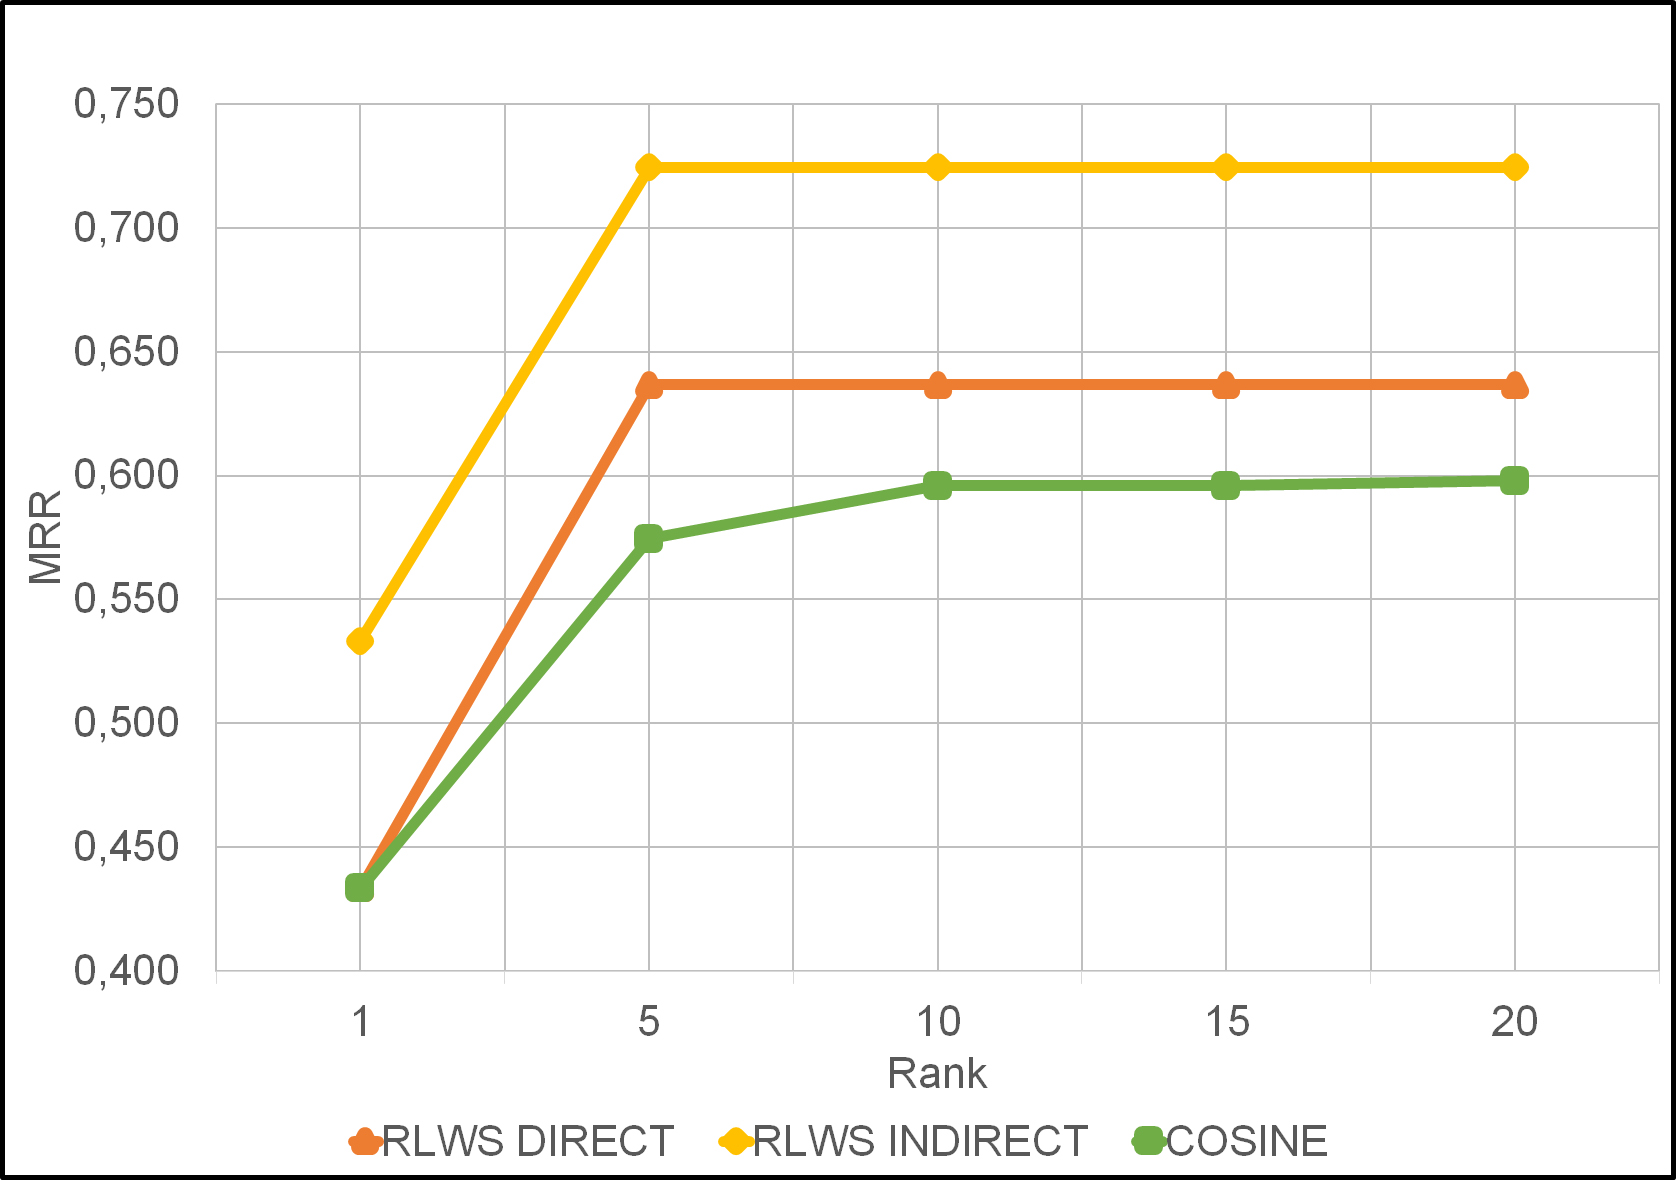
\includegraphics[width=.8\linewidth]{imagens/mrr_results_offline.jpg}
        \caption{testes offline}
        \label{fig:mrr_line_b}
    \end{subfigure}
    \caption{MRR - Gráfico com linhas dos três experimentos nos testes online e offline}
    \label{fig:mrr_line}
\end{figure}

\begin{figure}
    \begin{subfigure}{.5\textwidth}
        \centering
        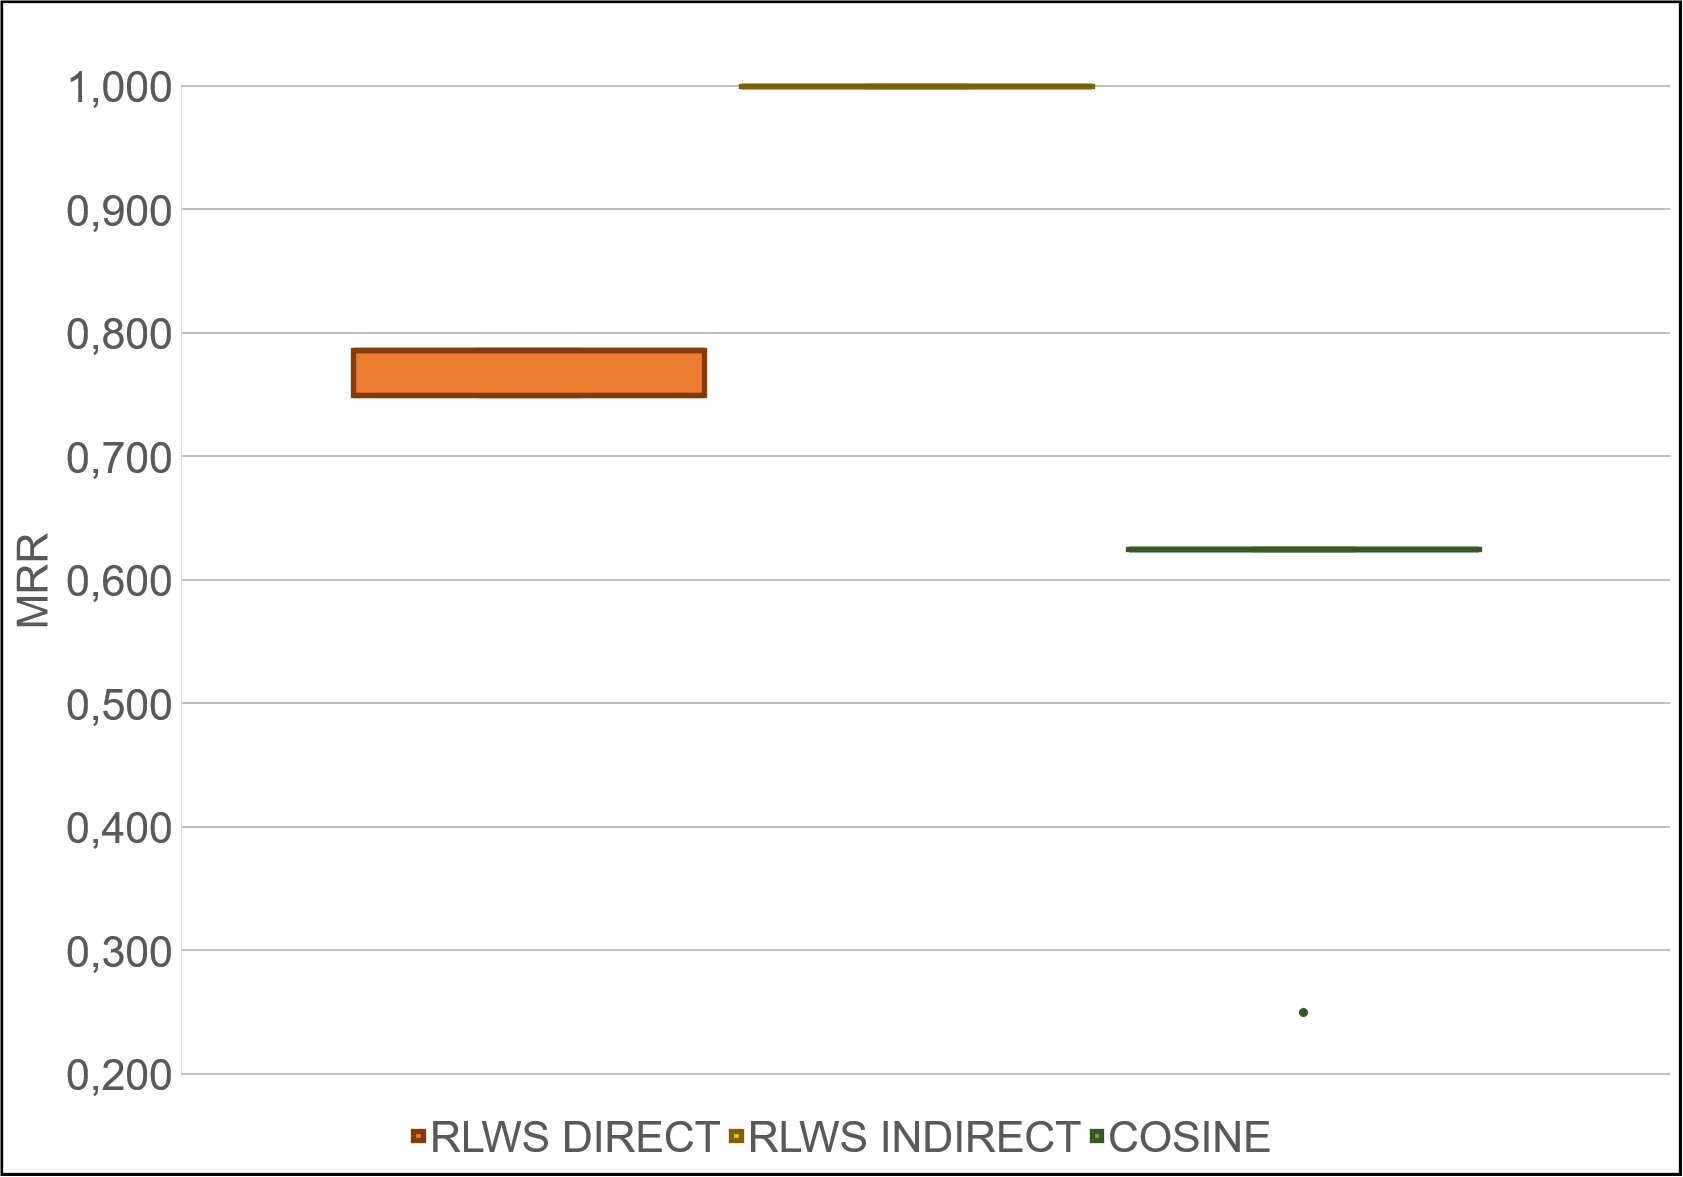
\includegraphics[width=.8\linewidth]{imagens/mrr_box_plot_online.jpg}
        \caption{testes online}
        \label{fig:mrr_box_plot_a}
    \end{subfigure}%
    \begin{subfigure}{.5\textwidth}
        \centering
        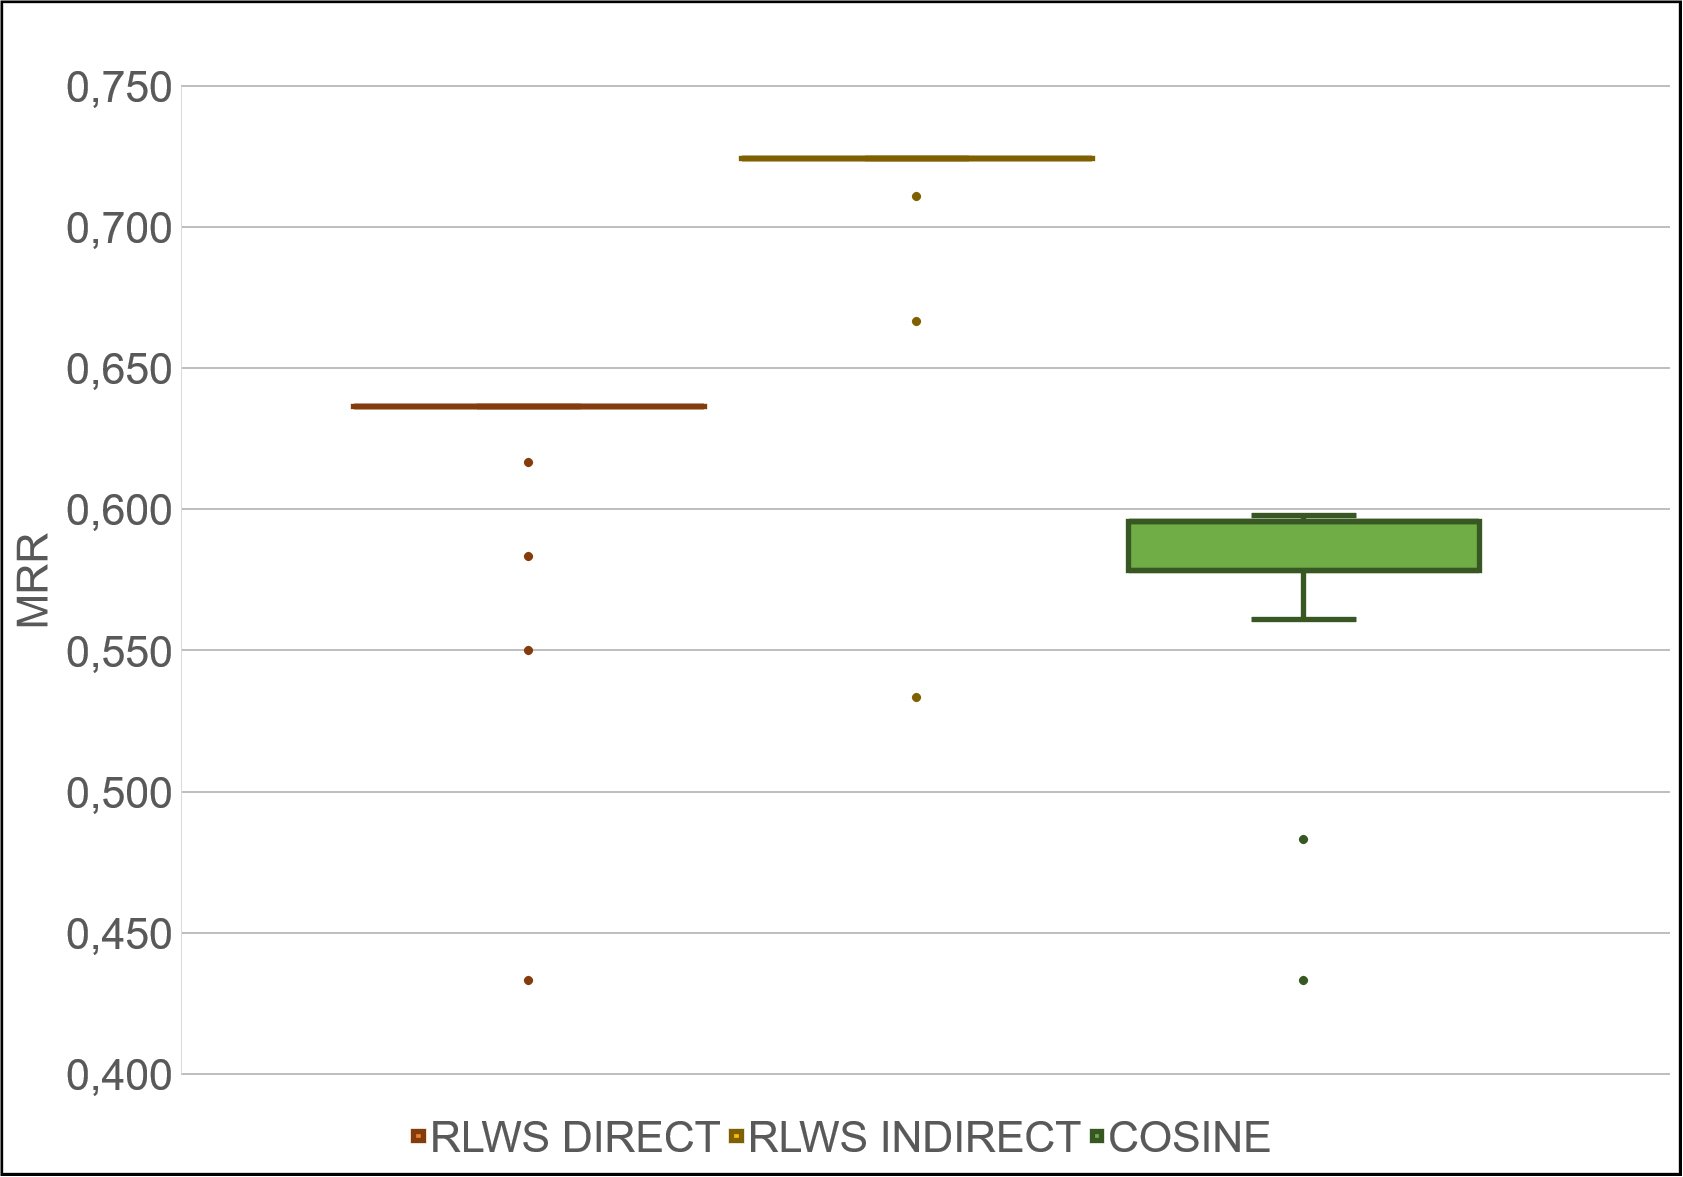
\includegraphics[width=.8\linewidth]{imagens/mrr_box_plot_offline.jpg}
        \caption{testes offline}
        \label{fig:mrr_box_plot_b}
    \end{subfigure}
    \caption{MRR - Gráfico de caixa dos três experimentos nos testes online e offline}
    \label{fig:mrr_box_plot}
\end{figure}

\section{Discussão dos resultados}

Utilizando as métricas apresentadas na metodologia foi possível observar que em especial ao uso de relacionamentos indiretos entre termos, obteve-se um resultado consideravelmente superior a métrica da similaridade do cosseno. Já quanto a variante \textbf{RLWS DIRECT}, obteve um resultado misto, sendo na maior parte das vezes superior em relação a métrica comparada. Ainda que com um grupo de testes limitado, os resultados indicam que é possível tirar proveito de uma análise semântica entre termos, podendo trazer resultados melhores de que uma análise sintática. Outra observação trata-se de que durante as entrevistas dos usuários nos testes \textit{online}, foi notado que o uso da descrição dos itens como \textit{feature} para construção do modelo de recomendação, aparentemente gerou recomendações que \enquote{fugiram à bolha tradicional} de resultados, algo que era um dos pontos do problema apresentado no capítulo \ref{cap:introducao}. Contudo, para um diversa quantidade de usuários o uso de certas \textit{features} dos itens, como ano de lançamento, gênero, autor ainda podem obter bons resultados, em especial de que é difícil avaliar se o modelo do usuário baseado na sinopse dos filmes, obtendo os termos mais relevantes, consegue captar corretamente suas preferências de narrativa, além de que o uso de outras características dos itens podem ser mais relevantes de usuário para usuário.

Outro ponto importante para ressaltar trata-se de que como o modelo de recomendação (ver seção \ref{ssec:rec_alg}) utiliza a descrição do item, um dado não estruturado, torna o sistema não muito dependente do domínio aplicado, sendo perfeitamente possível de ser utilizado numa recomendação para livros, por exemplo. Ainda que a similaridade semântica proposta seja intuitivamente coerente e de que é possível utilizá-la para modelar recomendações potencialmente mais precisas que métodos tradicionais, não seria tão adequada para comparações de textos grandes, sendo o objetivo para modelar um \ac{SR}, devido ao alto custo e carga de consultas a serem realizadas no DBPedia. Para comparar recursos individualmente ou uma coleção de palavras em pequenos textos, seria o uso mais indicado para tal similaridade.

\section{Pontos de melhorias}

Alguns desafios foram encontrados durante a construção do sistema de recomendação, principalmente relacionados a métrica de similaridade. Notou-se que a ambiguidade é um grande problema para análise de recursos na DBPedia\footnote{http://wiki.dbpedia.org}, inclusive ambiguidade em dois sentidos. O primeiro deve-se à ambiguidade no próprio serviço da web semântica que é vista pela propriedade \textit{dbo:wikiPageDisambiguates}, como no exemplo do termo \enquote{Paraná}, que pode ser resolvido para o estado brasileiro, rio ou clube de futebol. Quando uma pesquisa com termo ambíguo é realizada a contagem de links torna-se menos eficaz do que feita sabendo qual termo específico está se referindo. 

O segundo sentido de ambiguidade é a da gerada pela propriedade \textit{dbo:wikiPageRedirects}, que trata-se de como o termo é resolvido para seu nome final, comportando-se como \textit{alias}. Quando se busca um termo como \textit{Automobile}, o mesmo é redirecionado para \textit{Car} como \ac{URI} final, isso para todos os possíveis \enquote{sinônimos}. Ainda que no sistema sejam considerados termos iguais devido à análise de redirecionamentos entre si, quando se compara com outro termo, existe uma divergência para pior na contagem de links indiretos. Em futuros trabalhos poderá ser feito um ajuste nas consultas para que a contagem de links diretos e indiretos sejam mais precisas, diminuindo os problemas de ambiguidade.

O custo para se executar o modelo de recomendação proposto, é outro ponto de melhoria, pois ainda que o limite superior da complexidade de tempo seja $O(|Y| * |M_u| * |D_u|)$, dentro do esperado, o modelo do usuário e de filmes tendo um custo $|M_u| * |D_u|$, na prática torna-se um conjunto de termos grande para ser executado no DBPedia. É possível identificar este problema pela Equação \ref{eq:comb_term} que demonstra o cálculo de todas as combinações de termos possíveis, sendo $n$ o total de termos associados a \ac{URI}, que apenas utilizando os 5.107 filmes, foram encontrados 18630, resultado num total de 173.529.135 comparações possíveis. Ainda que este seja o limite teórico, e de que muitos termos não venham a ser comparados, é possível notar o quanto este número pode crescer rapidamente, sendo uma alta carga de comparações, mesmo utilizando \textit{multithreading}\footnote{Multithreading trata-se da possibilidade de trabalhar com múltiplas linhas execução concorrente, tornando um processamento de dados paralelo invés de linear.} e a estrutura de \textit{cache} da contagem de links proposta na seção \ref{sec:cache}.

\begin{equation}
	C(n, 2) = \frac{n!}{2!(n - 2)!}
\label{eq:comb_term}
\end{equation}

O objetivo não é alterar o custo dado pela equação das combinações, mas verificar maneiras de diminuir os modelos para recomendação, assim reduzindo a carga teórica de consultas no DBPedia. Inclusive este problema é um dos fatores que dificultaram a execução de testes com mais usuários, algo que precisa de mais tempo para ter um conjunto maior de comparações. Com essas melhorias realizadas nos modelos, será possível expandir mais facilmente os testes \textit{online}, inclusive relacionado a este ponto também facilitaria a construção de uma plataforma online na Web para que o usuário pudesse escolher suas preferências, exibindo as recomendações para que ele mesmo avalie, dispensando o uso de entrevistas.

Outra observação importante para melhorar, trata-se do cálculo com o modelo de recomendação, onde realiza-se uma simples média do $RLWS_{max, t_u}$ de cada termo $t_u$. A diferença do tamanho entre os modelos não é levada em conta, podendo então ser aplicado algum peso, como a frequência. Seria relevante aprofundar nessa comparação, estudando variações e formas semelhantes como a \ac{WMD}, que realiza um cálculo do "custo de transformação" de um conjunto de termos no outro, utilizando conceitos do problema do transporte \citep{Transporte:2016}. Uma variação poderia ser invés de utilizar uma métrica de distância como a \textit{word2vec} \citep{word2vec:2013}, aplicar uma que utilize similaridade (ou distância) semântica.

Um último ponto de melhoria trata-se do processo de \ac{NLP}, onde foram utilizados modelos pré-treinados oferecidos pela biblioteca \textit{OpenNLP}\footnote{https://opennlp.apache.org}. Com o uso deste modelo ocorreram diversas falhas ao reconhecer nomes de entidades (processo \ac{NER}). Para isso existem algumas possibilidades, como a de realizar um treinamento baseado nos textos dos filmes do próprio projeto, ou experimentar outras ferramentas como a \textit{Stanford CoreNLP}\footnote{https://stanfordnlp.github.io/CoreNLP/}.

\section{Sumário}

Neste capítulo foram apresentados os resultados obtidos com o sistema de recomendação construído, assim como uma análise da métrica de similaridade semântica. Para isso foram discutidas as metodologias junto com os dados utilizadas, além de estudadas as métricas que foram usadas nos resultados.